\documentclass[notitlepage, 12pt]{report} 

\usepackage{amsmath}
\usepackage{graphicx}
\usepackage{caption}
\usepackage[hidelinks]{hyperref}
\usepackage{circuitikz}[american]
\usepackage{booktabs}
\usepackage{graphicx}
\usepackage{listings}
\usepackage{pgfplots}
\usepackage{subcaption}

\usepackage[style=numeric]{biblatex}
\addbibresource{bib.bib}

\usepackage[top=2cm, bottom=2cm, left=2cm, right=2cm]{geometry}

\title{Final project}
\begin{document}

\begin{center}
\Large \textbf{Final Project: Audio Equalizer} \\
\small 
Ezekiel Ulrich \\
\date\\
009 (Nishant Thiagarajan)\\
\end{center}
\vspace{4in}

\begin{abstract}
\noindent This report details the design, construction, and testing of an adjustable audio equalizer circuit as 
part of ECE 20007's final project. 
The audio equalizer independently amplifies low ($0-320 Hz$), 
mid-range ($320-3200 Hz$), and high ($3200+ Hz$) frequencies. It must meet ripple, output power, and cutoff specifications.
In addition to measuring outputs with lab testing equipment, the circuit's performance 
is demonstrated with a live adjustment of input audio.
This project integrates many topics from previous labs, 
notably signal filtering and operational amplification. The report 
details the theoretical foundation of audio equalization and its component 
processes, outlines the procedure of design and construction, and presents 
the circuit valdiation results. These results are then discussed and the 
project's success in meeting specifications analyzed.  
\end{abstract}

\newpage

\section*{Introduction}
This project is the culmination of a semester's work, synthesizing 
passive/active filters and op-amps into a tangible demonstration: an adjustable 
audio equalizer capable of selectively modifying the frequencies 
of an input signal. The final circuit must accept a $320 mV$ RMS signal and selectively amplify 
frequencies in the ranges of 0-320, 320-3200, and $3200+ Hz$. These seperated
signals must be re-integrated and their aggregate independently amplified so that 
the output signal is suitable for driving a speaker. 
Additionally, the circuit must meet performance specifications for cutoff, 
ripple, and extremum amplification settings, as tabulated below. 
\begin{enumerate}
    \item \textbf{Cutoff:} each frequency must have a cutoff frequency
    (or in the case of the middle frequency filter, cutoff frequencies)
    within $10\%$ of the listed cutoff value. 
    \item \textbf{Ripple:} when each volume knob is turned to its maximum, 
    the difference between the highest peak and lowest trough 
    must be no greater than $15mV$. 
    \item \textbf{Extremum:} at each input frequency 
    indicated, the output RMS for each of the low, middle, and high 
    frequency filters set to minimum volume must be at most $15 mV$, 
    while the output RMS must be within $100 mV$ when set to maximum volume. 
    After summation, the output power must be greater than $400 mW$ when the 
    input signal is between $100$ and $10000 Hz$. 
\end{enumerate}
\begin{center}
    \begin{tabular}{c c} 
        \toprule
        Specification & Value \\
        \hline  
        Bass filter $-3dB$ cutoff & $320 Hz \pm 10\%$ \\
        Middle filter $-3dB$ cutoff & $320-3200 Hz \pm 10\%$ \\
        Treble filter $-3dB$ cutoff & $3200 Hz \pm 10\%$ \\
        \hline
        Maximum ripple & $15 mV RMS$ \\
        \hline
        Min output RMS & $15 mV$ \\
        Max output RMS & $100 mV \pm 10\%$ \\
        Min output power & $400 mW$ for $100-10000 Hz$ input \\
        \bottomrule  
    \end{tabular}
\end{center}

The significance of this project extends beyond its technical complexity. 
It serves as a bridge between theory and practice, drawing on concepts 
discussed in ECE 20001 as well as empirical observations in ECE 20007. 
As engineering endeavors progressively demand adeptness in translating 
theory to functional products, we must not merely meet technical specifications 
but foster passion for
the underlying science of what we design, so that we may always strive to learn 
and illuminate the dark corners of the universe. Thus, this project is the last in a 
series of stepping stones into a dark pond. From now on we must pick up the path
to move forward and take what we have seen with us as we progress ever farther 
into that vast expanse. Let us step bravely and lovingly into those unknown waters and
move beyond, with the hope that others may walk securely on the stones we lay behind.

\newpage

\section*{Theory}
As this project draws from several labs that have come before, 
an overview of the audio equalizer's subcircuits is
in order. Although many concepts and components from past work are present 
(capacitors, inductors, RMS voltage), we may identify two crucial constituents:
\textbf{passive filters} and \textbf{operational amplifiers}. 

\subsection*{Filters}
By combining resistors, inductors, and capcitors, we may create 
circuits that permit signals within a range of frequencies to pass 
unimpeded while attenuating frequencies outside this range. By carefully selecting 
values for the inductors and capacitors, we can adjust the permitted frequencies
to any range desired. Let us examine a type of passive filter which permits all 
frequencies below a specified cutoff, the RC low-pass filter shown in Figure 
\ref{fig:RClowpassfilter}. 
\begin{figure}
    \caption{RC low-pass filter}
    \label{fig:RClowpassfilter}
    \begin{center}
        \begin{circuitikz}
            \draw 
            (0,0) node[left] {$V_{in}$}
            to[R, l=$R_{LPF}$, o-] ++(2,0) coordinate (ur)
            to[short,-o] ++(1,0) 
            node[right] {$V_{out}$}
            (ur) to[C, l=$C_{LPF}$] ++(0,-2)
            node[ground] {}
            ;
        \end{circuitikz} 
    \end{center}
\end{figure}
If we recall the behavior of a capacitor, as frequency increases, the impedence 
decreases according to the formula 
\begin{equation}
    Z_C = \frac{1}{j \omega C}
\end{equation}
Thus, the higher the frequency of the input signal, the more of that signal the capacitor
diverts to ground. If we plot the output signal of the circuit in Figure \ref{fig:RClowpassfilter}
as a function of frequency, we obtain a graph similar to Figure \ref{fig:RClowpassFRA}. 
\begin{figure}
    \caption{Frequency Response of an RC Low-Pass Filter}
    \label{fig:RClowpassFRA}
    \begin{center}
        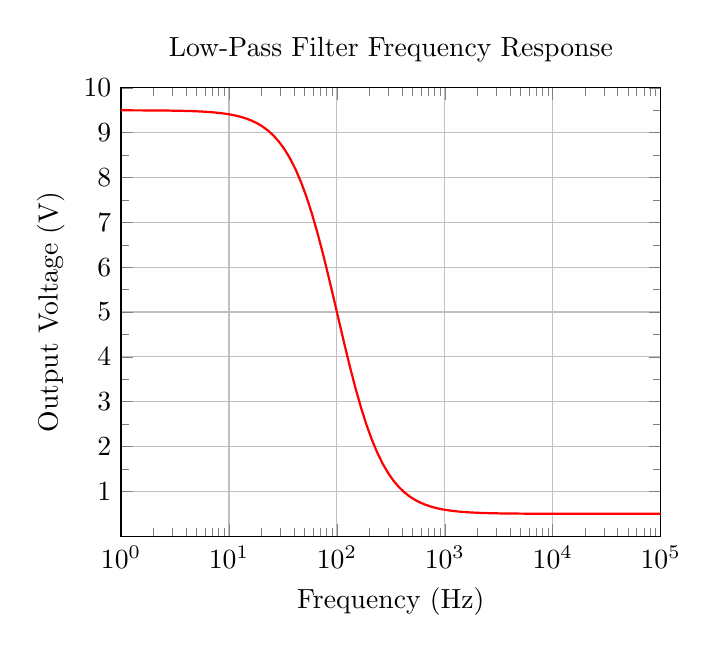
\begin{tikzpicture}
            \begin{axis}[
                xlabel={Frequency (Hz)},
                ylabel={Output Voltage (V)},
                title={Low-Pass Filter Frequency Response},
                grid=major,
                xmin=1, xmax=10^5,
                ymin=0, ymax=10,
                xmode=log,
                ytick={1,2,...,10},
                minor y tick num=1,
                legend pos=south east
            ]
            
            \addplot [domain=1:10^5, samples=100, red, thick] {-9*(x)^2/(100^2+(x)^2)+9.5};        
            \end{axis}
        \end{tikzpicture}
    \end{center}
\end{figure}
Typically, the signal cutoff frequency is defined as the frequency at which 
the gain $\frac{V_{out}}{V_{in}}$ is equal to $\frac{1}{\sqrt{2}}$, or on the decibel scale, 
the $-3dB$ point. We can analyze the circuit to determine precisely at what 
frequency this occurs. Notice that the circuit is set up in a voltage divider 
configuration, so the output voltage will be given by 
\begin{align}
    V_{out} &= V_{in} \times \frac{ - j X_C}{R_{LPF} - j X_C} \\
    &= V_{in} \times \frac{ - j X_C}{R_{LPF} - j X_C}.
\end{align}
Ergo, we have that 
\begin{align}
    \frac{V_{out}}{V_{in}} &= \frac{ - j X_C}{R_{LPF} - j X_C} \\
    \frac{1}{\sqrt{2}} &= \frac{ - j X_C}{R_{LPF} - j X_C} \\
    \frac{1}{\sqrt{2}} &= \left| \frac{ - j X_C}{R_{LPF} - j X_C} \right| \\
    &= \frac{X_C}{\sqrt{R_{LPF}^2 + X_C^2}} \\
    &= \frac{1}{ \sqrt{ \frac{R_{LPF}^2}{X_C^2} + 1} }
\end{align}
Therefore, we finally have 
\begin{align}
    \frac{R_{LPF}^2}{X_C^2} &= 1 \\
    R_{LPF} &= X_C \\
    &= \frac{1}{\omega C_{LPF}} \\
    \rightarrow \omega &= \frac{1}{R_{LPF} C_{LPF}} \\
    \rightarrow f_c &= \frac{1}{2 \pi R_{LPF} C_{LPF}}
\end{align}
With this process, we have found the specific frequency at 
which the gain is $\frac{1}{\sqrt{2}}$. We can repeat this process for 
any kind of filter, three different kinds of which this project uses. 
The other two are a RC high-pass filter (Figure \ref{fig:RChighpassfilter}, 
whose frequency response analysis graph is given in Figure \ref{fig:RChighpassFRA})
\begin{figure}
    \caption{RC high-pass filter}
    \label{fig:RChighpassfilter}
    \begin{center}
        \begin{circuitikz}
            \draw 
            (0,0) node[left] {$V_{in}$}
            to[C, l=$C_{HPF}$, o-] ++(2,0) coordinate (ur)
            to[short,-o] ++(1,0) 
            node[right] {$V_{out}$}
            (ur) to[R, l=$R_{HPF}$] ++(0,-2)
            node[ground] {}
            ;
        \end{circuitikz} 
    \end{center}
\end{figure}
\begin{figure}
    \caption{Frequency Response of an RC high-Pass Filter}
    \label{fig:RChighpassFRA}
    \begin{center}
        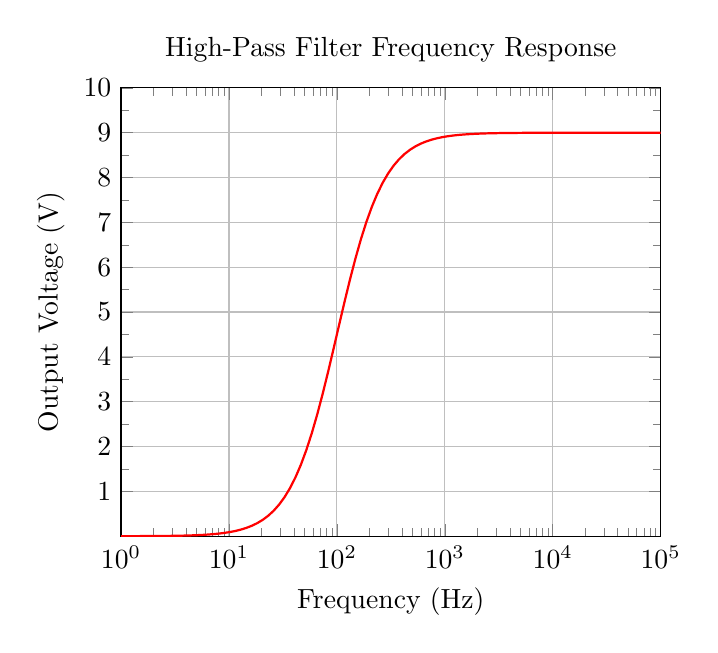
\begin{tikzpicture}
            \begin{axis}[
                xlabel={Frequency (Hz)},
                ylabel={Output Voltage (V)},
                title={High-Pass Filter Frequency Response},
                grid=major,
                xmin=1, xmax=10^5,
                ymin=0, ymax=10,
                xmode=log,
                ytick={1,2,...,10},
                minor y tick num=1,
                legend pos=south east
            ]
            
            \addplot [domain=1:10^5, samples=100, red, thick] {9*(x)^2/(100^2+(x)^2)};        
            \end{axis}
        \end{tikzpicture}
    \end{center}
\end{figure}
and a band-pass filter (Figure \ref{fig:RLCbandpassfilter}). 
\begin{figure}
    \caption{RLC band-pass filter}
    \label{fig:RLCbandpassfilter}
    \begin{center}
        \begin{circuitikz}
            \draw 
            (0,0) node[left] {$V_{in}$}
            to[L, l=$L_{BPF}$, o-] ++(2,0)
            to[C, l=$C_{BPF}$] ++(1,0) coordinate (ur)
            to[short, -o] ++(1,0)
            node[right] {$V_{out}$}
            (ur) to[R, l=$R_{BPF}$] ++(0,-2)
            node[ground] {}
            ;
        \end{circuitikz} 
    \end{center}
\end{figure}
The cutoff frequency of the RC high-pass filter, below which 
all frequencies are attenuated, is given by the same expression 
as the RC low-pass filter,
\begin{equation}
    f_c = \frac{1}{2 \pi R_{HPF} C_{HPF}}.
\end{equation}
The band-pass filter is different from the other two 
in that a range of frequencies are permitted, while outside
frequencies are not. Thus its characteristic 
equations take a different form. The frequency around which 
the pass band is centered (creatively called the \emph{center frequency}) is given by 
\begin{equation}
    f_C = \frac{1}{2 \pi \sqrt{L_{BPF} C_{BPF}}}. 
\end{equation}
The width of the pass band is given by the (equally creatively titled) \emph{bandwidth},
\begin{equation}
    \beta = \frac{R}{L}. 
\end{equation}
Thus, by tuning the values of $R_{HPF}$, $L_{HPF}$, and $C_{HPF}$ we 
may center and adjust the width of the pass band to whatever we desire. 
This project requires the use of all three filter types to seperate 
the frequencies into the $0-320$, $320-3200$, and $3200+Hz$ bands. 
Once seperated, these signals may be seperately amplified or attenuated
before recombination. Let us now turn to the component used to amplify 
signals, the \textbf{operational amplifer}. 

\subsection*{Amplifiers}
Operational amplifers, or \emph{op-amps}, accept two signals
and output one. Different combinations of op-amps and other 
components can achieve high gains ($10^5$ or more), isolate 
subcircuits to reduce loading, or sum many signals. The schematic 
for an op-amp is displayed in Figure \ref{fig:opampschematic}. 
\begin{figure}
    \caption{Operational amplifer schematic}
    \label{fig:opampschematic}
    \begin{center}
        \begin{circuitikz}
            \draw 
            (0,0) node[op amp] (opamp) {}
            (opamp.-) to[short] ++(-0.5,0)
            node[left] {inverting input, $v_-$}
            (opamp.+) to[short] ++(-0.5,0)
            node[left] {inverting input, $v_+$}
            (opamp.out) to[short] ++(0.5,0)
            node[right] {$V_{out}$}
            (opamp.down) to[short] ++(0,-0.5)
            node[below] {$V-$}
            (opamp.up) to[short] ++(0,0.5)
            node[above] {$V+$}
            ;
        \end{circuitikz}
    \end{center}
\end{figure}
The audio equalizer circuit in this project uses op-amps configured as 
inverting amplifers, whose layout is shown in Figure. \ref{fig:opampinvertingamp}. 
\begin{figure}
    \caption{Inverting amplifier schematic}
    \label{fig:opampinvertingamp}
    \begin{center}
        \begin{circuitikz}
            \draw (0,0) node[op amp] (op) {}

            (op.out) to[short] ++(0,1.5) 
            to[R, l=$R_2$] ++(-2.375,0)
            to[short] (op.-)

            (op.+) to[short] ++(0, -0.5)
            node[ground] {}

            (op.out) to[short] ++(0.5,0)
            node[right] {$v_{out}$}
            (op.-) to[short] ++(-0.2,0)
            to[R, l=$R_1$] ++(-1.5,0)
            node[left] {$v_{in}$}
            ;
        \end{circuitikz}
    \end{center}
\end{figure}
Application of Ohm's law at the inverting input terminal
reveals 
\begin{align}
    I_{R_1} &= \frac{v_{in} - v_-}{R_1} \\
    I_{R_2} &=  \frac{v_{out} - v_-}{R_2}  
\end{align}
Now, since $I_{R_1}$ and $I_{R_2}$ are the only currents 
delivered to the inverting input, Kirchhoff's current rule informs us that 
\begin{align}
    I_{R_1} + I_{R_2} &= 0 \\
    \frac{v_{in} - v_-}{R_1} + \frac{v_{out} - v_-}{R_2} &= 0 \\
    \frac{v_{in} - v_-}{R_1} &= -\frac{v_{out} - v_-}{R_2} \\
    (v_{in} - v_-)R_2 &= -(v_{out} - v_-)R_1 \\
    v_{in}R_2 - v_-R_2 &= -v_{out}R_1 + v_-R_1
\end{align}
Since the non-inverting input is grounded ($v_+ = 0$) and the op-amp is 
in a buffer configuration, we have that $v_- = 0$ and thus 
\begin{align}
    v_{in}R_2 - v_-R_2 &= -v_{out}R_1 + v_-R_1 \\
    v_{in}R_2 - 0\times R_2 &= -v_{out}R_1 + 0\times -R_1 \\
    v_{in}R_2 &= -v_{out}R_1 \\
    \frac{v_{out}}{v_{in}} &= -\frac{R_2}{R_1}
\end{align}
So by altering the ratio of $R_2$ to $R_1$, we may 
adjust the gain of the amplifier. This useful property finds application 
as a volume adjuster in the audio equalizer. By substituting a variable 
resistor in place of $R_2$, the gain of each frequency may be independently
controlled. The output of each is then fed into the input of another 
inverting amplifier, whose gain may be adjusted to control the volume of the 
entire output signal. 

\subsection*{Audio Equalizer}
Now that we are equipped with an understanding of the audio equalizer's 
fundemental components, let us integrate them and see how they adjust 
the different frequencies of an input signal. Once a singal of $320 mv$ RMS is 
connected, each filter will isolate its respective range of frequencies. 
The output of each filter then enters its amplifier, which allows for selective 
tuning. The amplified output is then recombined and fed into the master 
amplifier, whose amplification may be adjusted to control the volume of the entire signal. 
The signal then passes through the power amplifier and terminates in a speaker, where 
the effects of the equalization may be auditorily verified.  
The entire audio equalizer circuit schematic is displayed in Figure \ref{fig:equalizerschematic}. 
\begin{figure}
    \caption{Audio equalizer schematic}
    \label{fig:equalizerschematic}
    \begin{center}
        \scalebox{0.7}{
        \begin{circuitikz}

            % Coordinates 
            \coordinate (in) at (0,2);

            \coordinate (HPF) at (3,8);
            \coordinate (BPF) at (3,4);
            \coordinate (LPF) at (3,0);

            \coordinate (TVC) at (10,7.5);
            \coordinate (MVC) at (10,3.5);
            \coordinate (BVC) at (10,-0.5);
            \coordinate (OVC) at (16, 3);

            \coordinate (POW) at (17.8, 2.5);

            % Input signal
            \draw
            (in) node[ground] {}
            to[sV, l=$320 mv V_{RMS}$] ++(0,2)
            to[R, l=$50 \Omega$] ++(2,0) coordinate (inout)
            ;

            % High pass filter
            % (treble)
            \draw 
            (HPF) to[C, l=$C_{HPF}$] ++(2,0) coordinate (ur)
            to[short] ++(1,0) coordinate (hout)
            (ur) to[R, l=$R_{HPF}$] ++(0,-2)
            node[ground] {}
            ;

            % Band pass filter
            % (mid)
            \draw 
            (BPF) to[L, l=$L_{BPF}$] ++(2,0)
            to[C, l=$C_{BPF}$] ++(1,0) coordinate (ur)
            to[short] ++(1,0) coordinate (mout)
            (ur) to[R, l=$R_{BPF}$] ++(0,-2)
            node[ground] {}
            ;

            % Low pass filter
            % (bass)
            \draw 
            (LPF) to[R, l=$R_{LPF}$] ++(2,0) coordinate (ur)
            to[short] ++(1,0) coordinate (lout)
            (ur) to[C, l=$C_{LPF}$] ++(0,-2)
            node[ground] {}
            ;

            % Inverting op-amp
            % (treble volume control)
            \draw (TVC) node[op amp] (op) {}

            (op.out) to[short] ++(0,1.5) 
            to[vR] ++(-2.375,0)
            to[short] (op.-)

            (op.+) to[short] ++(0, -0.5)
            node[ground] {}

            (op.out) to[R, l=$R_{TVCout}$] ++(2,0) coordinate (tvcout)
            (op.-) to[short] ++(-0.2,0)
            to[R, l=$R_{TVCin}$] ++(-1.5,0) coordinate (tin)
            ;

            % Inverting op-amp
            % (mid volume control)
            \draw (MVC) node[op amp] (op) {}

            (op.out) to[short] ++(0,1.5) 
            to[vR] ++(-2.375,0)
            to[short] (op.-)

            (op.+) to[short] ++(0, -0.5)
            node[ground] {}

            (op.out) to[R, l=$R_{MVCout}$] ++(2,0) coordinate (mvcout)
            (op.-) to[short] ++(-0.2,0)
            to[R, l=$R_{MVCin}$] ++(-1.5,0) coordinate (min)
            ;

            % Inverting op-amp 
            % (bass volume control)
            \draw (BVC) node[op amp] (op) {}

            (op.out) to[short] ++(0,1.5) 
            to[vR] ++(-2.375,0)
            to[short] (op.-)

            (op.+) to[short] ++(0, -0.5)
            node[ground] {}

            (op.out) to[R, l=$R_{BVCout}$] ++(2,0) coordinate (bvcout)
            (op.-) to[short] ++(-0.2,0) 
            to[R, l=$R_{BVCin}$] ++(-1.5,0) coordinate (bin)
            ;

            % Inverting op-amp
            % (volume control)
            \draw (OVC) node[op amp] (op) {}

            (op.out) to[short] ++(0,1.5)
            to[vR] ++(-2.375,0)
            to[short] (op.-)

            (op.+) to[short] ++(0, -0.5)
            node[ground] {}

            (op.out) to[short] ++(0.62,0) coordinate (ovcout)
            (op.-) to[short] ++(-1,0) coordinate (ovcin)
            ;

            % Power amplifer 
            \draw 
            (POW) rectangle ++(2,1)
            node[above, right, yshift=0.5cm] at (POW) {LM386N4}
            ;

            % Wiring
            \draw  
            (inout) to[short] (BPF)
            to[short] (LPF)
            (BPF) to[short] (HPF)

            (hout) to[short] (tin)
            (mout) to[short] (min)
            (lout) to[short] (bin)

            (tvcout) to[short] (mvcout)
            (mvcout) to[short] (ovcin)
            (bvcout) to[short] (mvcout)

            (POW) to[short] ++(2,0)
            to[short] ++(0,0.5)
            to[short] ++(1,0) coordinate (out)
            to[R, l=Speaker ($8 \Omega$)] ++(0,-2)
            node[ground] {}
            (out) to[short, -o] ++(1,0) 
            node[right] {Out}
            ;
        \end{circuitikz}
        }
    \end{center}
\end{figure}


\pagebreak

\section*{Procedure}
With a firm basis of the underlying logic of the circuit, let's now 
step through how it was constructed. 
\begin{enumerate}
    \item First, values for the resistors, capacitors, and inductors were calculated as follows. 
    
    \emph{Low-pass filter specifications}: as seen in section Theory, the cutoff 
    frequency for a low-pass filter is given by 
    \[f_c = \frac{1}{2 \pi R_{HPF} C_{HPF}}.\]
    Since we require that $f_c = 320 Hz$, a capacitor value of $0.1 \mu C$ was chosen 
    for its availability in the minikit and a resistance of 
    \begin{align}
        R_{HPF} &= \frac{1}{2 \pi f_c C_{HPF}} \\
        &= \frac{1}{2 \pi (320 Hz) (0.1 \mu C)} \\
        &= 4973.59197162 \Omega \\
        &\approx 5.1 k\Omega
    \end{align}
    was calculated. The value was rounded to align with resistances provided in the minikit. 

    \emph{Band-pass filter specifications}: the center frequency for the band-pass filter is 
        \[f_C = \frac{1}{2 \pi \sqrt{L_{BPF} C_{BPF}}},\]
    while the bandwidth is 
        \[\beta = \frac{R}{L}.\]
    Our purposes require $f_c = 1760 Hz$ and $\beta = 2880 Hz$. Again, we select a 
    capacitor value before calculating resistance (and inductance). Let $C_{BPF} = 47 nF$, 
    then 
    \begin{align}
        L_{BPF} &= (\frac{1}{2\pi f_c})^2 \frac{1}{C_{BPF}} \\
        &= (\frac{1}{2\pi (1760 Hz)})^2 \frac{1}{47 nF} \\
        &= 0.173987108143 H \\
        &\approx 160 mH \\
        R &= \beta L_{BPF} \\
        &= 2880 Hz \times 0.160 H \\
        &= 460.8 \Omega \\
        &\approx 500 \Omega
    \end{align}
    
    \emph{High-pass filter specifications}: The formula for the cutoff frequency of a high-pass 
    filter is the same as that of the low-pass filter, 
        \[f_c = \frac{1}{2 \pi R_{HPF} C_{HPF}}.\]
    However, now $f_c = 3200$. We therefore again select the convenient $0.1 \mu C$ for the capacitor
    and find that 
    \begin{align}
        R_{HPF} &= \frac{1}{2 \pi f_c C_{HPF}} \\
        &= \frac{1}{2 \pi (3200 Hz) (0.1 \mu C)} \\
        &= 497.359197162 \Omega \\
        &\approx 500 \Omega
    \end{align}

    \emph{Amplifier specifications}: we know that the gain of an inverting 
    amplifier is given by 
        \[\frac{v_{out}}{v_{in}} = -\frac{R_2}{R_1}.\]
    Since the amplifier here needs to function as a volume control, the gain ought 
    to be between 0 and 1. We would also like to dynamically and conveniently adjust the volume, 
    for which we should use a potentiometer. Since the only potentiometer in the minikit 
    is $10 k\Omega$, we have that 
    \begin{align}
        R_1 &= -R_2 \frac{v_{in}}{v_{out}} \\
        &= 10 k\Omega
    \end{align}
    $R_2$, the potentiometer, may be tweaked to adjust the gain lower. 

    \emph{Output power}: We know to avoid loading we must make $R_{TVCout}$, $R_{MVCout}$, $R_{BVCout}$
    large in proportion to $R_{TVCin}$, $R_{MVCin}$, $R_{BVCin}$, which are all $10 k\Omega$. Let us choose 
    $R_{TVCout} = R_{MVCout} = R_{BVCout} = 100 k\Omega$. Simulation of the circuit then 
    reveals that the output voltage, without power amplification, is approximately $150 mV$ RMS at $3200 Hz$. 
    We require the final output power to be over $400 mW$ with an $8 \Omega$ speaker. Thus, the 
    output RMS voltage must be greater than 
    \begin{align*}
        V &= \sqrt{PR} \\
        &= \sqrt{400 mW 8 \Omega} \\
        &= \sqrt{3.2} V \\
        &\approx 1.789 V
    \end{align*}
    The gain of the LM386 is 20, which brings the pre-amplification $150mV$ RMS to $150mV \times 
    20 = 3 V$, well above the threshold of $1.789V$. 
    \item Next, the circuit outlined in Figure \ref{fig:equalizerschematic}
    was constructed in LTspice and simulated with a transient analysis to ensure functionality.
    Since LTspice lacks a native LM386 component, one was created and 
    inserted using code provided by user Jonk on StackExchange \cite{jonk}.
    \item Then, each subcircuit was created and independently tested in the following 
    order:
    \begin{enumerate}
        \item High-pass filter. Tested with frequency response analysis (FRA) on oscilloscope. 
        \item Band-pass filter. Tested with FRA. 
        \item Low-pass filter. Tested with FRA. 
        \item High-pass volume control. Tested with digital multimeter (DMM) and power supply unit (PSU). 
        \item Band-pass volume control. Tested with DMM and PSU. 
        \item Low-pass volume control. Tested with DMM and PSU. 
        \item Total volume control. Tested with DMM and PSU. 
        \item Power amplifier. Tested with DMM and PSU. 
    \end{enumerate}
    After each subcircuit was operational, it was integrated into the larger 
    audio equalizer. 
    \item Next, the circuit was judged on its ability to meet the benchmarkes outlined in the Introduction. 
    Measurements were gathered and compiled under Results. 
    \item Finally, the circuit was connected to an audio input and output. Sound was played
    and adjusted to confirm functionality. 
\end{enumerate}

\pagebreak

\section*{Results}

\subsection*{Spice Simulation}
The Spice schematic created for simulation is shown in 
Figure \ref{fig:spicesim}. 
\begin{figure}
    \caption{Spice schematic of audio equalizer}
    \label{fig:spicesim}
    \begin{center}
        \includegraphics[scale=0.5]{images/spicesim.png}
    \end{center}
\end{figure}
To demonstrate proper functionality of the circuit, 
it was shown that the filters worked as expected, the output power was sufficient 
for each, and that the volume may be adjusted as needed. 
\begin{enumerate}
    \item \emph{Filters}: Figure \ref{fig:spicesimresultsfreq} shows the simulated output
    \begin{figure}    
        \begin{subfigure}{0.3\textwidth}
            \includegraphics[scale=0.5]{images/spicesimresults320.png}
        \end{subfigure}\\
            \begin{subfigure}{0.3\textwidth}
            \includegraphics[scale=0.5]{images/spicesimresults3200.png}
        \end{subfigure}\\
        \begin{subfigure}{0.3\textwidth}
            \includegraphics[scale=0.5]{images/spicesimresults32000.png}
        \end{subfigure}    
    
        \caption{Spice simulation results at 320 (top), 3200 (middle), and 32000 (bottom) Hz input}
        \label{fig:spicesimresultsfreq}
    \end{figure}
    of each filter at frequencies of 320, 3200, and $32000Hz$. As can be seen from 
    the figure, each filter attenuates the signal below the $-3dB$ point at 
    its respective cutoff frequency. 
    \item \emph{Output voltage}: Figure \ref{fig:spicesimpower} shows the magnitude 
    of the output before and after amplification at the lowest frequency, $320 Hz$. 
    \begin{figure}    
        \begin{subfigure}{0.3\textwidth}
            \includegraphics[scale=0.5]{images/spiceunamplified.png}
        \end{subfigure}\\
            \begin{subfigure}{0.3\textwidth}
            \includegraphics[scale=0.5]{images/spiceamplified.png}
        \end{subfigure}\\
        \begin{subfigure}{0.3\textwidth}
            \includegraphics[scale=0.5]{images/spiceamplifiedandunamplified.png}
        \end{subfigure}    
    
        \caption{Output at $320 Hz$ for unamplified (top), amplified (middle), and both (bottom)}
        \label{fig:spicesimpower}
    \end{figure}
    It can be easily seen that amplification brings the voltage above the value 
    required to drive a speaker of $8 \Omega$, which was previously calculated as 
    $\approx 1.789 V$ RMS. 
    \item \emph{Volume control}: Figure \ref{fig:spicevolume} shows the output 
    \begin{figure}    
        \begin{subfigure}{0.3\textwidth}
            \includegraphics[scale=0.5]{images/volume011.png}
        \end{subfigure}
            \begin{subfigure}{0.3\textwidth}
            \includegraphics[scale=0.5]{images/volume101.png}
        \end{subfigure}
        \begin{subfigure}{0.3\textwidth}
            \includegraphics[scale=0.5]{images/volume110.png}
        \end{subfigure} 
        
        \begin{subfigure}{\textwidth}
            \centering
            \includegraphics[width=0.6\linewidth]{images/volume000.png}
        \end{subfigure}
    
        \caption{0 volume for HPF (left), BPF (middle), LPF (right), and all (bottom)}
        \label{fig:spicevolume}
    \end{figure}
    signals at each of the three volume controls, as well as the complete output volume. 
    As the figure shows, when all three volume controls are turned down, the output 
    voltage is on the order of nanovolts. When one is turned down, its corresponding 
    output is so small in relation to the others as to seem flat on the graph. 
\end{enumerate}

\subsection*{Empirical Analysis}
The following aspects of the circuit were tested: filters, output voltage at minimum volume, 
output voltage at maximum volume, total volume control, signal recombination, ripple, and output power.  
\begin{enumerate}
    \item \emph{Filters}: Figure \ref{fig:frafilters} shows the measured output
    \begin{figure}    
        \begin{subfigure}{0.3\textwidth}
            \includegraphics[scale=0.2]{images/lowpass.png}
        \end{subfigure}
        \hfill
        \begin{subfigure}{0.3\textwidth}
            \includegraphics[scale=0.2]{images/bandpass.png}
        \end{subfigure}
        \hfill
        \begin{subfigure}{0.3\textwidth}
            \includegraphics[scale=0.2]{images/highpass.png}
        \end{subfigure}    
    
        \caption{FRA results for low-pass (left), band-pass (middle), and high-pass (right) filters}
        \label{fig:frafilters}
    \end{figure}
    of each filter at frequencies of 200, 2000, and $10000Hz$ (the upper limit of human hearing).
    \item \emph{Output RMS voltage at minimum volume}: Figure \ref{fig:minvolume} shows 
    \begin{figure}    
        \begin{subfigure}{0.3\textwidth}
            \includegraphics[scale=0.2]{images/minvollow.png}
        \end{subfigure}
        \hfill
        \begin{subfigure}{0.3\textwidth}
            \includegraphics[scale=0.2]{images/minvolmed.png}
        \end{subfigure}
        \hfill
        \begin{subfigure}{0.3\textwidth}
            \includegraphics[scale=0.2]{images/minvolhigh.png}
        \end{subfigure}    
    
        \caption{Output signal with minimum volume for 200, 2000, and $10000Hz$}
        \label{fig:minvolume}
    \end{figure}
    the magnitude of the output signal at a range of frequencies when the master volume dial is 
    turned to a minimum.
    \item \emph{Output RMS voltage at maximum volume}: Figure \ref{fig:maxvolume} shows the RMS values 
    \begin{figure}    
        \begin{subfigure}{0.3\textwidth}
            \includegraphics[scale=0.2]{images/maxvollow.png}
        \end{subfigure}
        \hfill
        \begin{subfigure}{0.3\textwidth}
            \includegraphics[scale=0.2]{images/maxvolmed.png}
        \end{subfigure}
        \hfill
        \begin{subfigure}{0.3\textwidth}
            \includegraphics[scale=0.2]{images/maxvolhigh.png}
        \end{subfigure}    
    
        \caption{Output signal with maximum volume for 200, 2000, and $10000Hz$}
        \label{fig:maxvolume}
    \end{figure}
    of the voltage feeding into the power amplifer when the volume control is set to max. 
    \item \emph{Volume control}: Figure \ref{fig:volume} displays the output signal with the 
    \begin{figure}    
        \begin{subfigure}{0.3\textwidth}
            \includegraphics[scale=0.2]{images/lowvolume.png}
        \end{subfigure}
        \hfill
        \begin{subfigure}{0.3\textwidth}
            \includegraphics[scale=0.2]{images/medvolume.png}
        \end{subfigure}
        \hfill
        \begin{subfigure}{0.3\textwidth}
            \includegraphics[scale=0.2]{images/highvolume.png}
        \end{subfigure}    
    
        \caption{Input and output signal for low (left), medium (middle), and high (right) volume}
        \label{fig:volume}
    \end{figure}
    volume control at zero, turned slightly, and turned to the max.
    \item \emph{Signal recombination}: Figure \ref{fig:signalsummation} shows three input signals
    \begin{figure}    
        \begin{center}
            \includegraphics[scale=0.4]{images/addedsignals.png}  
        \end{center}
        \caption{Input signals to each filter and recombined output}
        \label{fig:signalsummation}
    \end{figure}
    to each of the three filters: a since wave, triangle wave, and square wave.
    \item \emph{Ripple}: Figure \ref{fig:ripple} displays the gain at maximum volume during FRA.
    \begin{figure}    
        \begin{center}
            \includegraphics[scale=0.4]{images/ripple.png}  
        \end{center}
        \caption{Gain at maximum volume across frequency range}
        \label{fig:ripple}
    \end{figure}
    \item \emph{Output power}: Figure \ref{fig:outputpower} displays the RMS voltage of the circuit. 
    \begin{figure}    
        \begin{center}
            \includegraphics[scale=0.4]{images/outputpower.png}  
        \end{center}
        \caption{Output RMS voltage}
        \label{fig:outputpower}
    \end{figure}
\end{enumerate}

\pagebreak

\section*{Discussion}

The project is a resounding success, meeting and in many cases significantly exceeding benchmarks 
on all tests: filtering, output voltages at minimum and maximum volumes, volume control functionality, 
signal recombination, ripple control, and output power. 
\begin{enumerate}
    \item \emph{Filters}: As can be seen from Figure \ref{fig:frafilters}, each filter 
    attenuates the signal below the $-3dB$ point at its respective cutoff frequency. 
    \item \emph{Output RMS voltage at minimum volume}: As Figure \ref{fig:minvolume} shows, 
    the output at minimum volume is on the order of $\mu V$ for all frequencies, 
    which would be inaudible for most humans. 
    \item \emph{Output RMS voltage at maximum volume}: The RMS values must be $100 mVRMS \pm 10 \%$, 
    and our observed values are $95.09 mV$, $98.64 mV$, 
    and $109.20 mV$. Although the latter value approaches the 10 \% threshold, all values are  
    within and therefore satisfy the requirement. 
    \item \emph{Volume control}: As can be qualitatively seen in Figure \ref{fig:volume}, 
    the volume varies according to the degree at which the master volume knob is turned. 
    \item \emph{Signal recombination}: As Figure \ref{fig:signalsummation} shows, the combined 
    graph displays the output of the summing inverting amplifier and represents a superposition 
    of these waves with combined characteristics of the three input waves, showing proper signal 
    summation. 

    \item \emph{Ripple}: Figure \ref{fig:ripple} shows the gain at maximum volume during is mostly
    linear with a maximum difference of $0.78 dB$. That means 
    that the human ear will percieve a roughly 10\% difference in loudness between the frequency 
    which produces the lowest gain and the frequency which produces the highest. This is 
    absolutely acceptable and will barely be perceptible when listening to music from the 
    audio equalizer. 
    \item \emph{Output power}: Figure \ref{fig:outputpower} shows that the RMS voltage of the circuit 
    is $2.052 V$. With an $8\Omega$ speaker, this produces a power of
    \begin{align*}
        P &= \frac{V_{RMS^2}}{R} \\
        &= \frac{(2.052 V)^2}{8 \Omega} \\
        &= 0.526338 W \\
        &= 526.338 mW \\
        &>400 mW
    \end{align*}
    Since we exceed the power needed to drive the speaker, this requirement, too, is met. 
\end{enumerate}
Overall, these findings affirm the device's functionality, precision, and compliance with specifications, 
validating its potential for effective audio signal processing.

\section*{Conclusion}

Now we are done. This report has exhaustively detailed the theory, simulation, 
construction, and testing of an audio equalizer. The circuit successfully 
filtered the input signal into the desired frequency bands, 
used inverting op-amps to attentuate select frequencies, 
recombined these signals while allowing for further volume adjustment, 
and amplified the result so that it could drive a speaker with measured specifications. 

This rock has been heaved into place, and the path behind us is a bit longer now. Perhaps 
in some time we will walk it again. If we do it will be as builders with new eyes 
and new minds, for returning to where we began is not the same as never leaving. 


\printbibliography[title={\Large References}]

\end{document}